\section{Supporting Materials}
% ==================================================================================================
\subsection{Notation}\label{app.notation}
Table~\ref{tab:notation} summarizes our notation,
and any corresponding parameters from \cite{Arenas2020}.
\begin{table}[ht]
  \centering
  \caption{Notation}
  \begin{tabular}{ccl}
  \toprule
   Symbol   &        Symbol        & Definition                     \\
   in this  & in \cite{Arenas2020} &                                \\
  \midrule
     $g$    &         $i$          & home patch                     \\
    $g'$    &         $j$          & other patch                    \\
    $g^*$   &         ---          & visited patch                  \\
     $a$    &         $g$          & self age group                 \\
    $a'$    &         $h$          & other age group                \\
     $y$    &         ---          & contact type                   \\
     $n$    &         ---          & home FSA                       \\
    $n'$    &         ---          & visited FSA                    \\
     $i$    &         $m$          & infection state                \\
     $P$    &         $N$          & population size                \\
     $B$    &         $R$          & mobility matrix                \\
     ---    &         $M$          & convenience mobility matrix    \\
  $\lambda$ &        $\Pi$         & force of infection             \\
   $\rho$   &         $p$          & mobility factor                \\
     $h$    &         ---          & home pool contact proportion   \\
     $C$    &         $k$          & contacts per person            \\
     $X$    &         ---          & total absolute contacts        \\
  $\theta$  &         $C$          & contacts age distribution      \\
   $\phi$   &         ---          & odds of mobility if unobserved \\
   $\psi$   &         ---          & relative time away from home   \\
  \bottomrule
\end{tabular}
  
  \label{tab:notation}
\end{table}
% ==================================================================================================
\subsection{Interpretation of ``Non-mobile''}\label{app.non-mob}
As described in \S~\ref{meth.orig}, \citet{Arenas2020} model the degree of mobility of age group $a$
using a parameter $\rho_a$ (our notation),
incorporated into a convenience matrix $M_{gg'}$ per Eq.~(\ref{eq:Arenas.M})\,/\,(\ref{eq:Arenas.M.app}),
repeated here for reference:
\begin{equation}\label{eq:Arenas.M.app}
  M_{gg'a} = (1-\rho_a)\,\delta_{gg'} + \rho_a B_{gg'a}
\end{equation}
The implicit assumption of this approach is that
non-mobile individuals may form contacts with visitors to the former's residence patch
(situation~\ref{situ:mob-at-home} in \S~\ref{meth.prop.mix.mob}):
an assumption which may not be desired depending on the research question or intervention effect.
The proposed approach to modelling mixing can avoid this assumption if needed
through the use of ``home pools'' (situation~\ref{situ:non-mob}).
Figure~\ref{fig:nm} explores the potential influence of
compulsory mixing of non-mobile individuals with mobile visitors on network connectivity,
as measured by the expected proportion of contacts formed with other patches, in a toy example.
The example has 3 patches, each having equal population size and random mobility ($B_{gg'} = 1/N_{g'}$).
Age is not considered.
\par
By simulating mixing between non-mobile individuals and mobile visitors,
as described in issue~\ref{issue:mobility}
(Figures \ref{fig:nm.half.stay}~\&~\ref{fig:nm.diff.stay}, situation~\ref{situ:mob-at-home})
the proportions of contact made with other patches increases for all patches,
as compared to the proposed approach
(Figures \ref{fig:nm.half.home}~\&~\ref{fig:nm.diff.home}, situation~\ref{situ:non-mob}).
The difference is largest in the context of differential mobility by patch
% SM: here, refer to issue 2? and also could refer back to its implications
%     v. briefly (differential mobility by age, but also other contexts...)
% JK: @SM I guess it kind of includes both issues
%     2 (different age mixing by contact type) and
%     3 (whether non-mobile mix with visitors),
%     but I've added an implication sentence next; hopefully it helps?
(Figures~\ref{fig:nm.diff.stay}~vs~\ref{fig:nm.diff.home}).
Thus, the original approach could underestimate
the transmission reduction impacts of reduced mobility,
especially when some patches can reduce mobility-related mixing while others cannot.
\par
\begin{figure}[ht]
  \newcommand{\threepct}[3]{#1,~#2,~#3\,\%}
  \centering
  \begin{subfigure}{0.49\linewidth}
    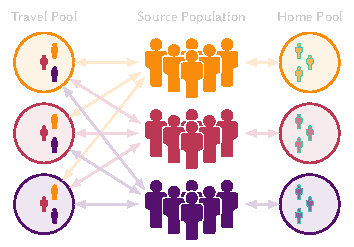
\includegraphics[width=\linewidth]{pools-half-home}
    \caption{Non-mobile = stay at home, all patches 50\% mobile}
    \label{fig:nm.half.home}
    \floatfoot{Contacts formed with other patches:\\
      33\% if non-mobile have equal contact rates vs mobile\\
      44\% if non-mobile have 1/2 contact rates vs mobile}
  \end{subfigure}\hfill%
  \begin{subfigure}{0.49\linewidth}
    \centering
    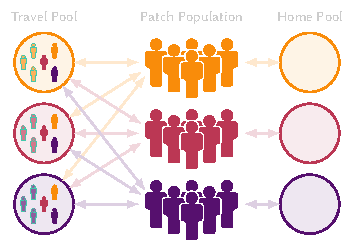
\includegraphics[width=\linewidth]{pools-half-stay}
    \caption{Non-mobile = stay in patch, all patches 50\% mobile}
    \label{fig:nm.half.stay}
    \floatfoot{Contacts formed with other patches:\\
      50\% if non-mobile have equal contact rates vs mobile\\
      59\% if non-mobile have 1/2 contact rates vs mobile}
  \end{subfigure}\medskip\par
  \begin{subfigure}{0.49\linewidth}
    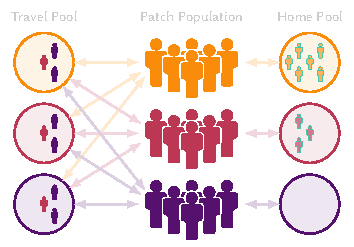
\includegraphics[width=\linewidth]{pools-diff-home}
    \caption{Non-mobile = stay at home, patches \threepct{0}{50}{100} mobile}
    \label{fig:nm.diff.home}
    \floatfoot{Contacts formed with other patches:\\
      \threepct{0}{33}{33} if non-mobile have equal contact rates vs mobile\\
      \threepct{0}{44}{33} if non-mobile have 1/2 contact rates vs mobile}
  \end{subfigure}\hfill%
  \begin{subfigure}{0.49\linewidth}
    \centering
    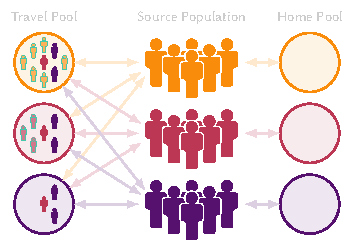
\includegraphics[width=\linewidth]{pools-diff-stay}
    \caption{Non-mobile = stay in patch, patches \threepct{0}{50}{100} mobile}
    \label{fig:nm.diff.stay}
    \floatfoot{Contacts formed with other patches:\\
      \threepct{33}{48}{59} if non-mobile have equal contact rates vs mobile\\
      \threepct{50}{58}{52} if non-mobile have 1/2 contact rates vs mobile}
  \end{subfigure}
  \caption{Mixing implications for two assumptions about
    the behaviour of non-mobile populations (issue~\ref{issue:mobility}):
    ``stay at home'' (\subref{fig:nm.half.home},\subref{fig:nm.diff.home},
    reflecting situation~\ref{situ:non-mob}):
    % SM: in main text, sometimes referred to as issue 3, etc...
    %     suggest either situation or issue for consistency...
    % JK: @SM I would say the three situations from 2.2.2 all pertain to
    %     the proposed solution to issue #3 (how changes to mobility are modelled) from 2.1,
    %     so I reference both here now -- does that work?
    no contacts with other patches (proposed here); vs
    ``stay within patch'' (\subref{fig:nm.half.stay},\subref{fig:nm.diff.stay},
    reflecting situation~\ref{situ:mob-at-home}):
    no travel, but may form contacts with travellers from other patches (as~in~\cite{Arenas2020}).}
  \floatfoot{
    Non-mobile populations are indicated with faded colour and green outline;
    patch-specific values ordered from top (yellow) to bottom (purple).
    Additional assumptions:
    large population size;
    equal population sizes and contact rates by patch;
    random mobility (equal probability of visiting any patch if mobile).}
  \label{fig:nm}
  \vspace{-5ex} % TEMP
\end{figure}
\clearpage
% ==================================================================================================
\subsection{Deriving the Mobility Matrix: Example}\label{app.mob}
% JK: @SM big re-writes to this section to reflect the latest data from AG
%     (% away time within home FSA)
%     and corresponding changes to the methodology incorporating the new data
Here we describe the methods used to obtain the mobility matrix $B_{gg'}$
for our applied example in Ontario Canada (details in \S~\ref{ex}).
The mobility matrix represents
the expected proportions of individuals residing in decile (patch) $g$ who travel to decile $g'$ each day.
% --------------------------------------------------------------------------------------------------
\subsubsection{Data}\label{app.mob.data}
The data are from a private anonymized database representing
approximately 2\% of mobile devices in Ontario.%
\footnote{\hreftt{https://www.veraset.com}}
The raw data represent logs of: unique device ID, timestamp, and geolocation
(latitude\,/\,longitude, with accuracies of meters to tens of meters).
A log entry (``ping'') is generated when an app on the device
requests the current geolocation from the service provider.
The geolocation is compared to:
a) boundary files representing all 513 Ontario FSAs%
\footnote{\hreftt{https://www150.statcan.gc.ca/n1/en/catalogue/92-179-X}}
to determine which FSA the ping is attributed to; and
%b) Geohash-6 tiles (1.2 \,km $\times$ 609.4\,m)
b) Geohash-7 tiles (152.9\,m $\times$ 152.4\,m)
to help identify the approximate home location.
The following definitions were then used in determining device mobility.
\begin{itemize}
  \item \textbf{Home dwelling:} for each unique device, the Geohash-6 tile with
  the greatest total evening time (8:00\,pm--5:00\,am) each calendar month.
  Devices for which it was not possible to determine the home dwelling
  were excluded from all further analysis.
  \item \textbf{Home FSA:} for each device, the FSA containing
  the midpoint of the home dwelling Geohash-6 tile.
  \item \textbf{Visited FSA:} FSAs that a device travelled to within a 24-hour period,
  as defined by at least 2 consecutive pings spanning at least 2 hours within the FSA.
  By this definition, it was possible for a device to visit
  multiple FSAs, or no FSA during a given day.
  Repeated visits to the same FSA by the same device on the same calendar date
  are treated as a single visit.
  \item \textbf{Time away from home:} for each device,
  the proportion of total time spent away from the home dwelling.
  Only devices with at least 5 pings spanning at least 4 hours were included.
  \item \textbf{Time away from home within home FSA:} for each device,
  the proportion of total time spent away from the home dwelling but still within the home FSA.
\end{itemize}
\par
These definitions were applied to each calendar month $t$ from Jan 2020--Dec 2020 (12 months) to compute:
the mean number of devices with home FSA $n$ per day, denoted $H_{nt}$ or ``observed devices'';
the mean number of devices with home FSA $n$ that visited FSA $n'$ per day, denoted $V_{nn't}$, or ``device visits'';
the mean proportion of time each device spent outside the home per day for each FSA, denoted $\Psi_{nt}$; and
the mean proportion of time each device spent outside the home but within the home FSA per day for each FSA, denoted $\Psi^h_{nt}$
% --------------------------------------------------------------------------------------------------
\subsubsection{Mobility Matrix}\label{app.mob.matrix}
The inter-FSA mobility matrix $B_{nn't}$ ($n \ne n'$) could be defined as
the expected proportion of observed devices that travelled to each FSA per day ($V_{nn't} / H_{nt}$).
However, the following analysis of the data suggested that such an approach may bias estimates of mobility.
A reference period $t_0$ was defined as Jan--Feb 2020, to reflect pre-pandemic conditions.
The expected values of $H_{nt}$ and $V_{nt} = \sum_{n'}V_{nn't}$ for each FSA $n$ during this period
were then computed and compared to the expected values during each subsequent month.
Figure~\ref{fig:RHVt} plots the distribution of ratios
$H_{nt} / H_{nt_0}$ (\subref{fig:RHt}) and $V_{nt} / V_{nt_0}$ (\subref{fig:RVt})
across all 513 FSAs, for each month.
These ratios illustrate that both $V_{nt}$ and $H_{nt}$ were influenced (reduced) by pandemic restrictions,
and thus $V_{nn't} / H_{nt}$ would overestimate mobility.
The trend in $H_{nt}$ might be because apps accessing geolocation services are only opened
after the user intends to travel, such as map-related apps.
As such, we term this bias ``mobility-intention bias''.
\begin{figure}
  \centering
  \begin{subfigure}[t]{0.45\linewidth}
    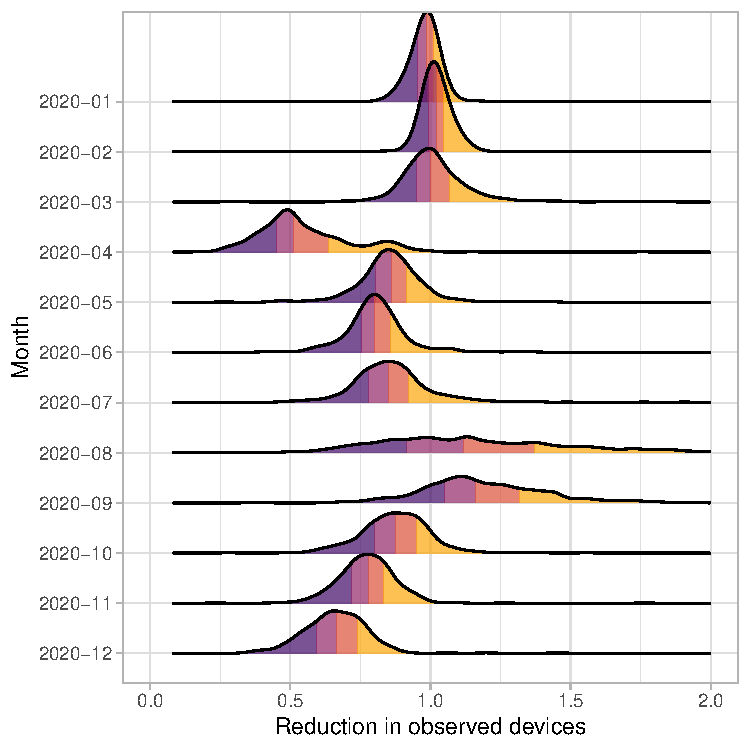
\includegraphics[width=\linewidth]{RHt}
    \caption{Observed devices at home}
    \label{fig:RHt}
  \end{subfigure}\quad
  \begin{subfigure}[t]{0.45\linewidth}
    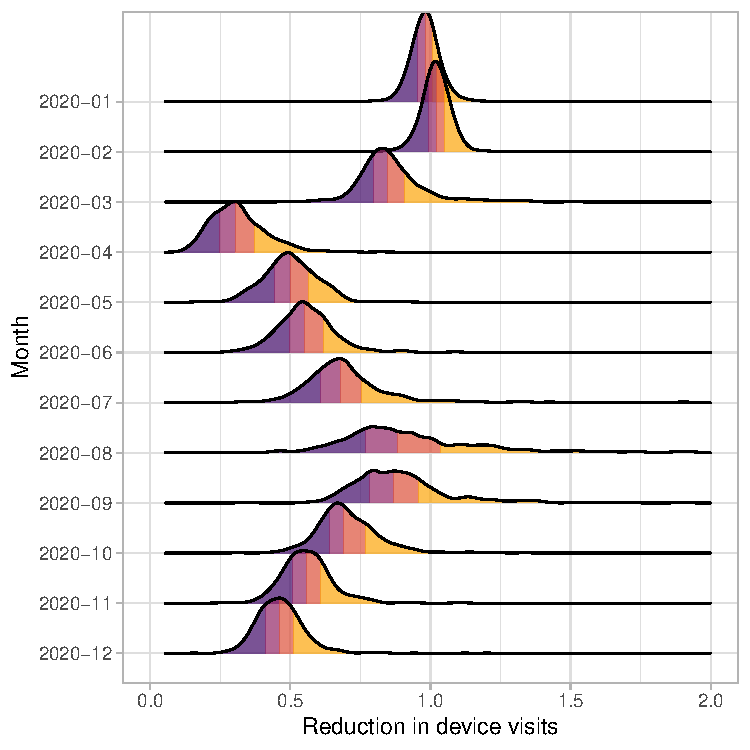
\includegraphics[width=\linewidth]{RVt}
    \caption{Total device visits}
    \label{fig:RVt}
  \end{subfigure}
  \caption{Ratios of (\subref{fig:RHt}) observed devices at home
    and (\subref{fig:RVt}) total device visits
    during each month versus during the reference period
    suggesting that the proportion of observed devices travelling each month
    alone is not reflective of true mobility or else (\subref{fig:RHt}) would be 1}
  \label{fig:RHVt}
  \floatfoot{Data from approximately 2\% of mobile devices in Ontario, Canada;
    distributions show the density of ratio values across all 513 FSAs;
    coloured segments indicate the 4 quantiles of each distributions;
    reference period: Jan--Feb 2020.}
\end{figure}
\par
To address the mobility-intention bias, we
separated the probability of an individual being mobile overall $\rho_{nt}$ from
the conditional probability of travelling to FSA $n'$
given that the individual is going to travel outside their home FSA $B^c_{nn't}$.
We defined this conditional probability of visiting FSA $n'$,
given that the individual is travelling outside the home FSA as:
\begin{equation}
  B^c_{nn't} = \frac{V_{nn't}}{\sum_{n'} V_{nn't}},\quad n \ne n'
\end{equation}
which no longer considers the total number of devices observed $H_{nt}$.
We then aggregated $B^c_{nn't}$ to obtain $B^c_{gg't}$
as noted in \S~\ref{ex:data}:
\begin{equation}\label{eq:Bgg.app}
  B^c_{gg't} = \sum_{n \in S_g}\sum_{n' \in S_g'} B^c_{nn't}
\end{equation}
where $S_g$ is the set of FSAs ($n$) corresponding to decile $g$.
\par
Next, we defined the overall probability of being mobile outside the home
for individuals from FSA $n$ during month $t$ as:
\begin{equation}
  \rho_{nt} = \frac{\Psi_{nt}}{\Psi_{nt_0}}
\end{equation}
reflecting an assumption that
100\% of individuals are mobile outside the home during the reference period~$t_0$,
and thus $\rho_{nt}$ represents a relative reduction from this baseline.
This definition of $\rho_{nt}$ aims to avoid the mobility-intention bias
because it is not directly affected by the numbers of observed devices each month
($V_{nn't}$ and/or $H_{nt}$), but rather
the behaviour (relative change in time away from home) associated with those devices.
Even if observed devices are more mobile than unobserved devices,
we think the reduction in time away from home relative to $t_0$
among observed devices/individuals
would be reasonably representative of the reduction
among unobserved devices/individuals.
\par
Similar to $\rho_{nt}$, we then defined
the proportion of time away from home spent within the home FSA as:
\begin{equation}
  \phi_{nt} = \frac{\Psi^h_{nt}}{\Psi_{nt}}
\end{equation}
Figure~\ref{fig:t-away} illustrates the distribution of
$\rho_{nt}$ (\subref{fig:rho-gt}) and
$\phi_{nt}$ (\subref{fig:phi-gt})
across different FSAs, stratified by month and decile.
We observe that the lower incidence deciles had
the lowest relative reduction in mobility $\rho_{nt}$ (\subref{fig:rho-gt}),
and sometimes had greater mobility during the pandemic as compared to the reference period.
We also observe that the majority of time spent away from home
is spent within the home FSA $\phi_{nt}$,
and that individuals in the lowest incidence deciles
spent the most time outside their home FSA (\subref{fig:phi-gt}).
We aggregate $\rho_{nt}$ and $\phi_{nt}$ for each decile $g$
using the mean across corresponding FSA $n$ to yield $\rho_{gt}$ and $\phi_{gt}$.
\begin{figure}
  \centering
  \begin{subfigure}[t]{0.45\linewidth}
    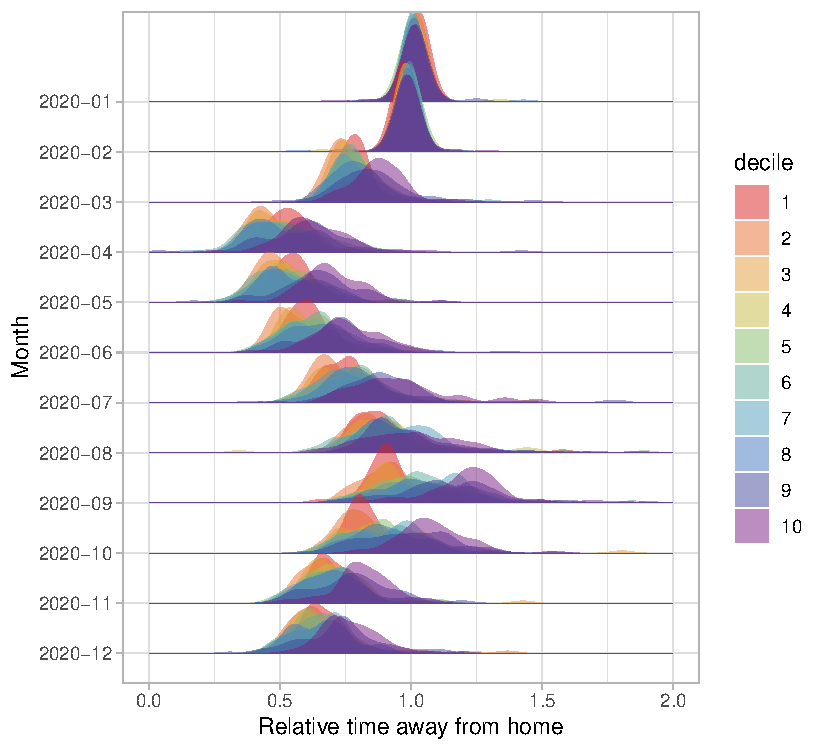
\includegraphics[width=\linewidth]{rho-gnt}
    \caption{Proportion of time away from home relative to the reference period
      ($\rho_{nt}$)}
    \label{fig:rho-gt}
  \end{subfigure}\quad
  \begin{subfigure}[t]{0.45\linewidth}
    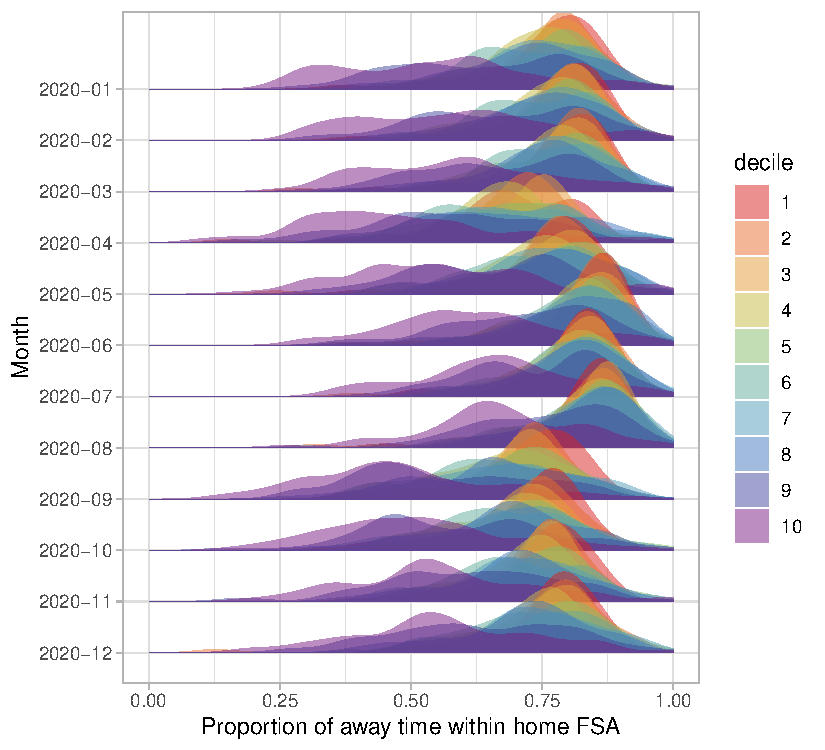
\includegraphics[width=\linewidth]{phi-gnt}
    \caption{Proportion of time away spent within the home FSA
      ($\phi_{nt}$)}
    \label{fig:phi-gt}
  \end{subfigure}
  \caption{Measures of time away from home used to calculate the mobility matrix}
  \label{fig:t-away}
  \floatfoot{Data from approximately 2\% of mobile devices in Ontario, Canada;
    distributions show the density of ratio values across all 513 FSAs;
    reference period: Jan--Feb 2020.}
\end{figure}
\par
Finally, we define the overall mobility matrix $B_{ggt}$ as
\begin{equation}\label{eq:Bgg.t}
  B_{gg't} = \rho_{gt} \Big[
    (\phi_{gt}) \delta_{gg'} + (1-\phi_{gt}) B^c_{gg't}
  \Big]
\end{equation}
representing a weighted average of
the identity matrix $\delta_{gg'}$ and
the conditional mobility matrix $B^c_{gg't}$, weighted by
intra-FSA mobility ($\phi_{gt}$) and
inter-FSA mobility ($1 - \phi_{gt}$), respectively,
and overall proportional to $\rho_{nt}$.
% --------------------------------------------------------------------------------------------------
\subsubsection{Dimensionality Reduction}\label{app.mob.reduce}
% JK: @SM this section completely new -- and possibly out of scope,
%     but the work needed to get done for the hotspot modelling,
%     so might as well write it up...
As written, Eq.~(\ref{eq:Bgg.t}) requires an additional observation of
$B^c_{gg't}$, $\phi_{gt}$, and $\rho_{gt}$ for each month $t$.
If any retrospective data are missing,
or for projecting $B_{gg't}$ into the future,
we are interested to know whether any of these three parameters
can be extrapolated based on a subset of the original inputs.
\par
First, we explored whether
the conditional distribution of mobility destinations $B^c_{gg't}$
could be replaced by the mean across months:
\begin{equation}\label{eq:Bc-approx}
  B^c_{gg'} = \frac{1}{N_t} B^c_{gg't}
\end{equation}
Figure~\ref{fig:Bc} plots the elements ($g,g'$) of $B^c_{gg't}$,
showing the time trend (\subref{fig:Bc-t})
and overall distribution of values (\subref{fig:Bc-box}).
Variation in $B^c_{gg't}$ between months was relatively small
(coefficients of variation were:
median~[min~(IRQ)~max] = 5.4~[2.4~(4.2,~8.2)~37.9]\%\,)
suggesting that the conditional probabilities for each month
could indeed be replaced by the mean as in Eq.~(\ref{eq:Bc-approx}).
\begin{figure}[ht]
  \begin{subfigure}{\linewidth}
    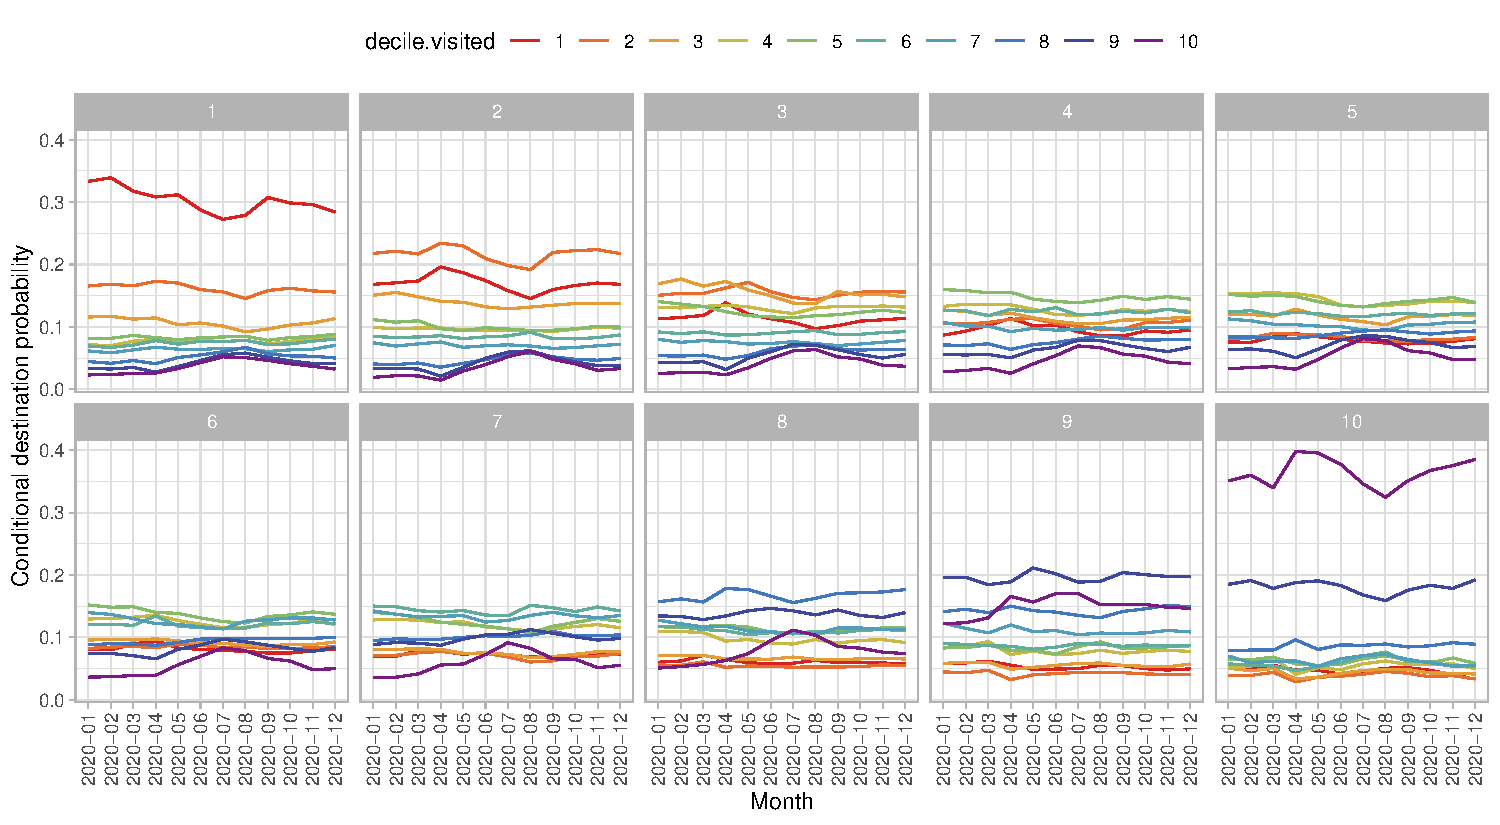
\includegraphics[width=\linewidth]{Bc-t}
    \caption{Trend versus month}
    \label{fig:Bc-t}
  \end{subfigure}
  \begin{subfigure}{\linewidth}
    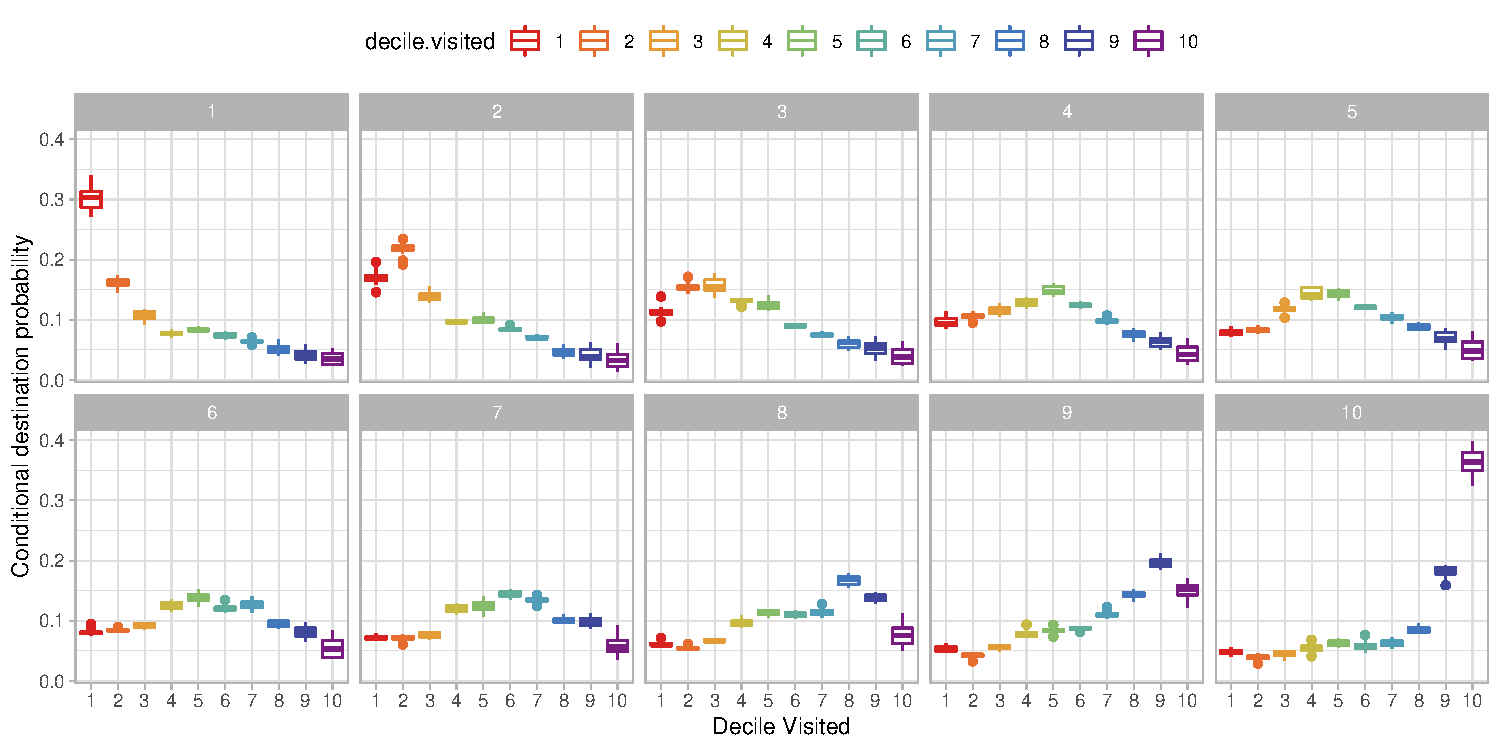
\includegraphics[width=\linewidth]{Bc-box}
    \caption{Distribution of conditional probabilities}
    \label{fig:Bc-box}
  \end{subfigure}
  \caption{Conditional probabilities of
    travelling from decile $g$ (panels) to decile $g'$ (colours) for Jan--Dec 2020,
    showing relative stability of conditional probabilities over time}
  \label{fig:Bc}
  \floatfoot{Data from approximately 2\% of mobile devices in Ontario, Canada.}
\end{figure}
\par
Next, we explored whether the proportion of time away from home
for each group and month could be replaced by
the mean for each month $\rho_{t}$and a relative group effect $R^{\,\rho}_{g}$:
\begin{equation}\label{eq:rho-gt-approx}
  \rho_{gt} \approx \rho_{t}\,R^{\,\rho}_{g}
\end{equation}
Figure~\ref{fig:rho} plots the mean $\rho_{t}$ for each month,
and the relative difference $R^{\,\rho}_{g} = \rho_{gt} / \rho_{t}$.
Again, variation between months in $R^{\,\rho}_{g}$ was small
(coefficients of variation: 2.8~[1.6~(2.0,~3.6)~4.2]\%\,)
suggesting that the approximation Eq.~(\ref{eq:rho-gt-approx}) is reasonable.
We ignore the pre-\covid reference period for estimating $R^{\,\rho}_{g}$,
as relative mobility $\rho_{gt} = 1$ by definition during this period.
\begin{figure}[ht]
  \begin{subfigure}[t]{0.297\linewidth}
    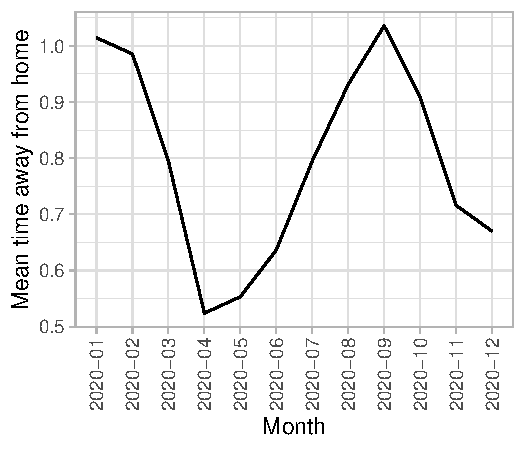
\includegraphics[width=\linewidth]{rho-t}
    \caption{Trend versus month: average mobility probability ($\rho_{t}$)}
    \label{fig:rho-t}
  \end{subfigure}\hfill
  \begin{subfigure}[t]{0.33\linewidth}
    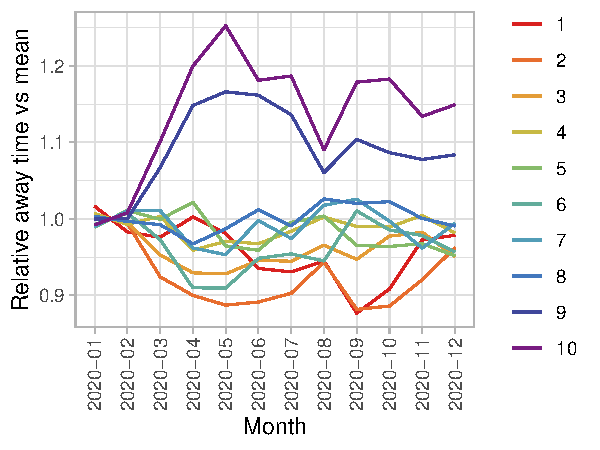
\includegraphics[width=\linewidth]{R-rho-gt}
    \caption{Trend versus month: relative differences in mobility by decile ($\rho_{gt} / \rho_{t}$)}
    \label{fig:rho-gt}
  \end{subfigure}\hfill
  \begin{subfigure}[t]{0.33\linewidth}
    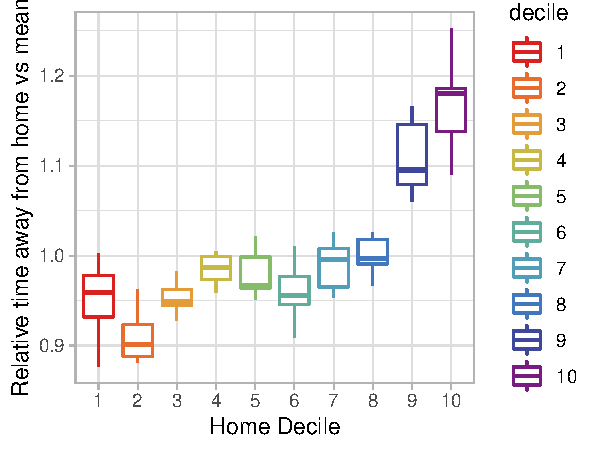
\includegraphics[width=\linewidth]{R-rho-box}
    \caption{Distribution of relative differences\,* ($\rho_{gt} / \rho_{t}$)}
    \label{fig:rho-box}
  \end{subfigure}
  \caption{Probability of being mobile for each decile $\rho_{gt}$
    versus the population average,
    showing relative stability over time}
  \label{fig:rho}
  \floatfoot{
    *\,During March--Dec 2020 only;
    data from approximately 2\% of mobile devices in Ontario, Canada.}
\end{figure}
\par
Finally, we likewise explored whether the ``intra-FSA mobility''
(proportion of away time spent within the home FSA)
for each group and month could be replaced by
the mean for each month $\phi_{t}$and a relative group effect $R^{\,\phi}_{g}$:
\begin{equation}\label{eq:phi-gt-approx}
  \phi_{gt} \approx \phi_{t}\,R^{\,\phi}_{g}
\end{equation}
Figure~\ref{fig:rho} plots the mean $\phi_{t}$ for each month,
and the relative difference $R^{\,\phi}_{g} = \phi_{gt} / \phi_{t}$.
Again, variation between months in $R^{\,\phi}_{g}$ was small
(coefficients of variation: 1.3~[0.8~(1.1,~2.5)~4.4]\%\,)
suggesting that the approximation Eq.~(\ref{eq:phi-gt-approx}) is also reasonable.
Since data on overall mobility $\rho_{t}$ may be easier to obtain or approximate than
the proportion of away time spent within the home FSA $\phi_{t}$,
we may also be interested to remove the time component of $\phi_{t}$ and use fixed $\phi$;
in this case the approximation is worse, but still very reasonable
(coefficients of variation: 7.2~[5.1~(6.5,~7.7)~11.2]\%\,).%
\footnote{It would also be helpful if $\phi_{t}$ could be predicted by $\rho_{t}$,
  but comparing the plots (Figures~\ref{fig:rho-t}~and~\ref{fig:phi-t}),
  we see they are poorly correlated.}
\begin{figure}[ht]
  \begin{subfigure}[t]{0.297\linewidth}
    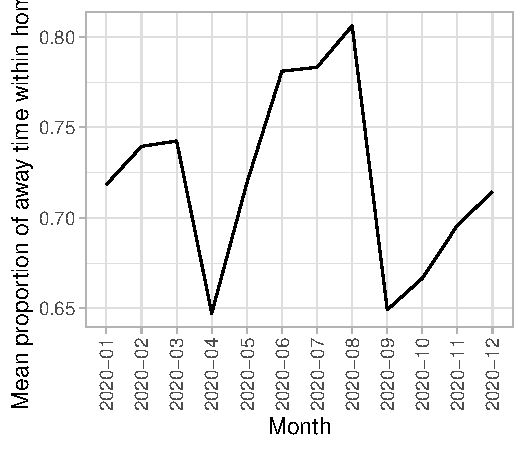
\includegraphics[width=\linewidth]{phi-t}
    \caption{Trend versus month: average mobility probability ($\phi_{t}$)}
    \label{fig:phi-t}
  \end{subfigure}\hfill
  \begin{subfigure}[t]{0.33\linewidth}
    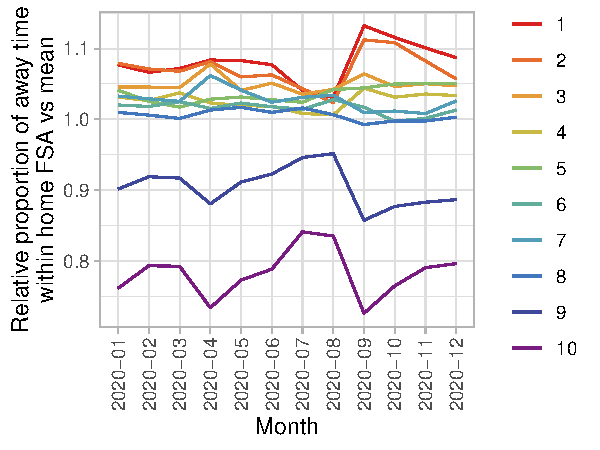
\includegraphics[width=\linewidth]{R-phi-gt}
    \caption{Trend versus month: relative differences in mobility by decile ($\phi_{gt} / \phi_{t}$)}
    \label{fig:phi-gt}
  \end{subfigure}\hfill
  \begin{subfigure}[t]{0.33\linewidth}
    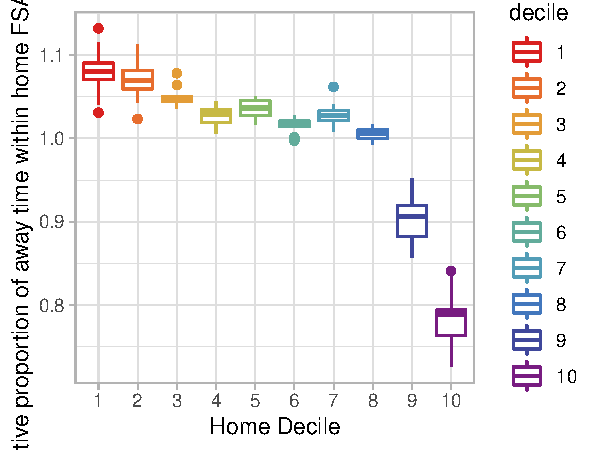
\includegraphics[width=\linewidth]{R-phi-box}
    \caption{Distribution of relative differences ($\phi_{gt} / \phi_{t}$)}
    \label{fig:phi-box}
  \end{subfigure}
  \caption{Conditional probability of intra-FSA mobility for each decile $\phi_{gt}$
    versus the population average,
    showing relative stability over time}
  \label{fig:phi}
  \floatfoot{
    Data from approximately 2\% of mobile devices in Ontario, Canada.}
\end{figure}
\par
Thus, overall Eq.(\ref{eq:Bgg.t}) can be re-written as:
\begin{equation}\label{eq:Bgg.t.approx}
  B_{gg't} \approx \rho_{t} R^{\,\rho}_{g} \Big[
    (\phi_{(t)}\,R^{\,\phi}_{g}) \delta_{gg'} + (1-\phi_{(t)}\,R^{\,\phi}_{g}) B^c_{gg't}
  \Big]
\end{equation}
where $\rho_{t}$, and possibly $\phi_{t}$, are the only required inputs.
Using the simpler approximation with fixed $\phi$, Figure~\ref{fig:Bggt}
compares (\subref{fig:Bggt-orig}) the unapproximated mobility matrix from Eq.~(\ref{eq:Bgg.t})
with (\subref{fig:Bggt-approx}) the approximated mobility matrix from Eq.~(\ref{eq:Bgg.t.approx}).
\begin{figure}[ht]
  \begin{subfigure}{\linewidth}
    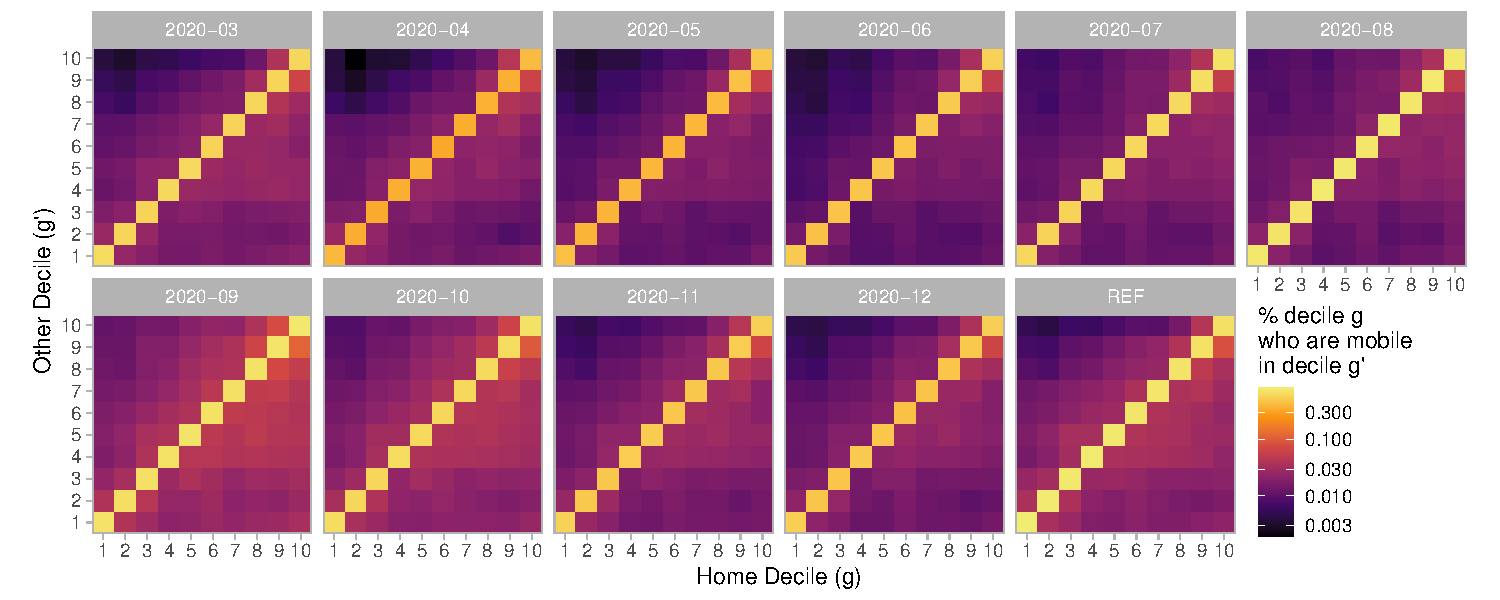
\includegraphics[width=\linewidth]{Bggt-log}
    \caption{Observed}
    \label{fig:Bggt-orig}
  \end{subfigure}
  \begin{subfigure}{\linewidth}
    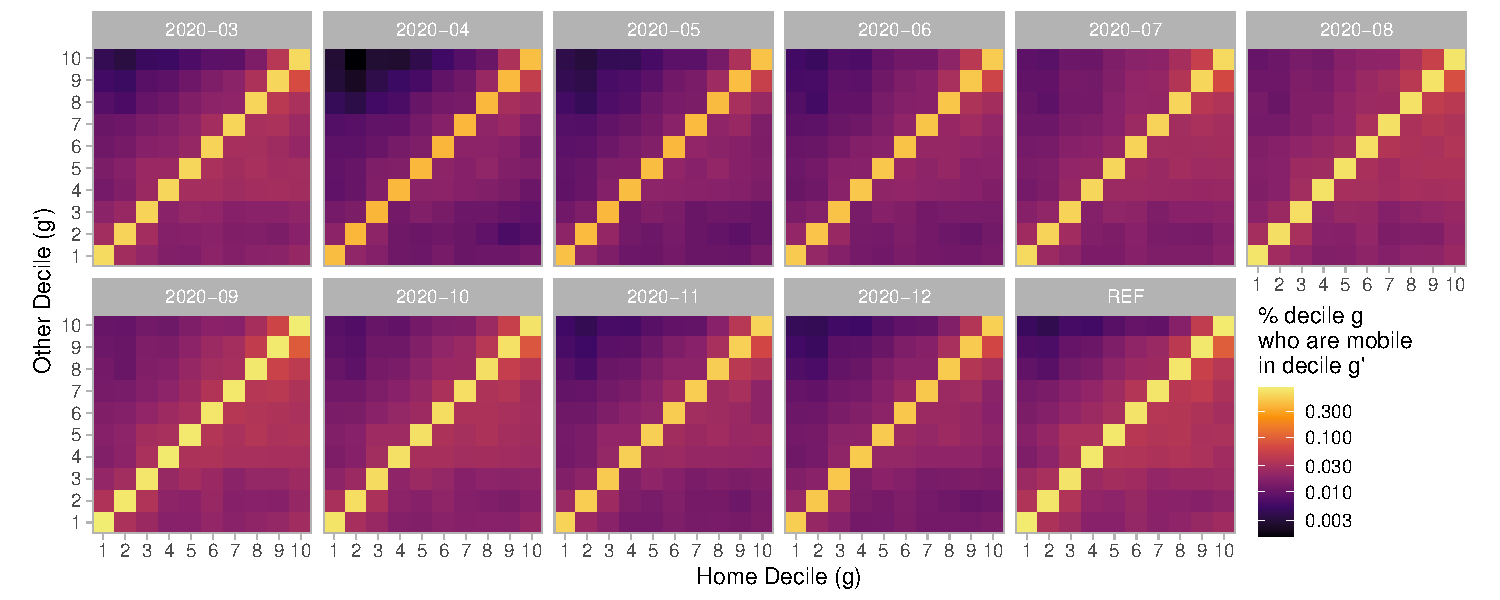
\includegraphics[width=\linewidth]{Baggt-log}
    \caption{Approximated}
    \label{fig:Bggt-approx}
  \end{subfigure}
  \caption{Visual comparison of
    observed mobility matrix $B_{gg't}$, Eq.~(\ref{eq:Bgg.t}) and
    approximated mobility matrix, Eq.~(\ref{eq:Bgg.t.approx})}
  \label{fig:Bggt}
  \floatfoot{Derived from mobile device geolocation data;
    deciles represent groupings of Ontario forward sortation areas (FSAs)
    by cumulative \covid cases between 15 Jan 2020--28 Mar 2021;
    colour scale is square-root transformed to improve perception of smaller values;
    reference period: Jan--Feb 2020.}
\end{figure}
\begin{figure}[ht]
  \centering
  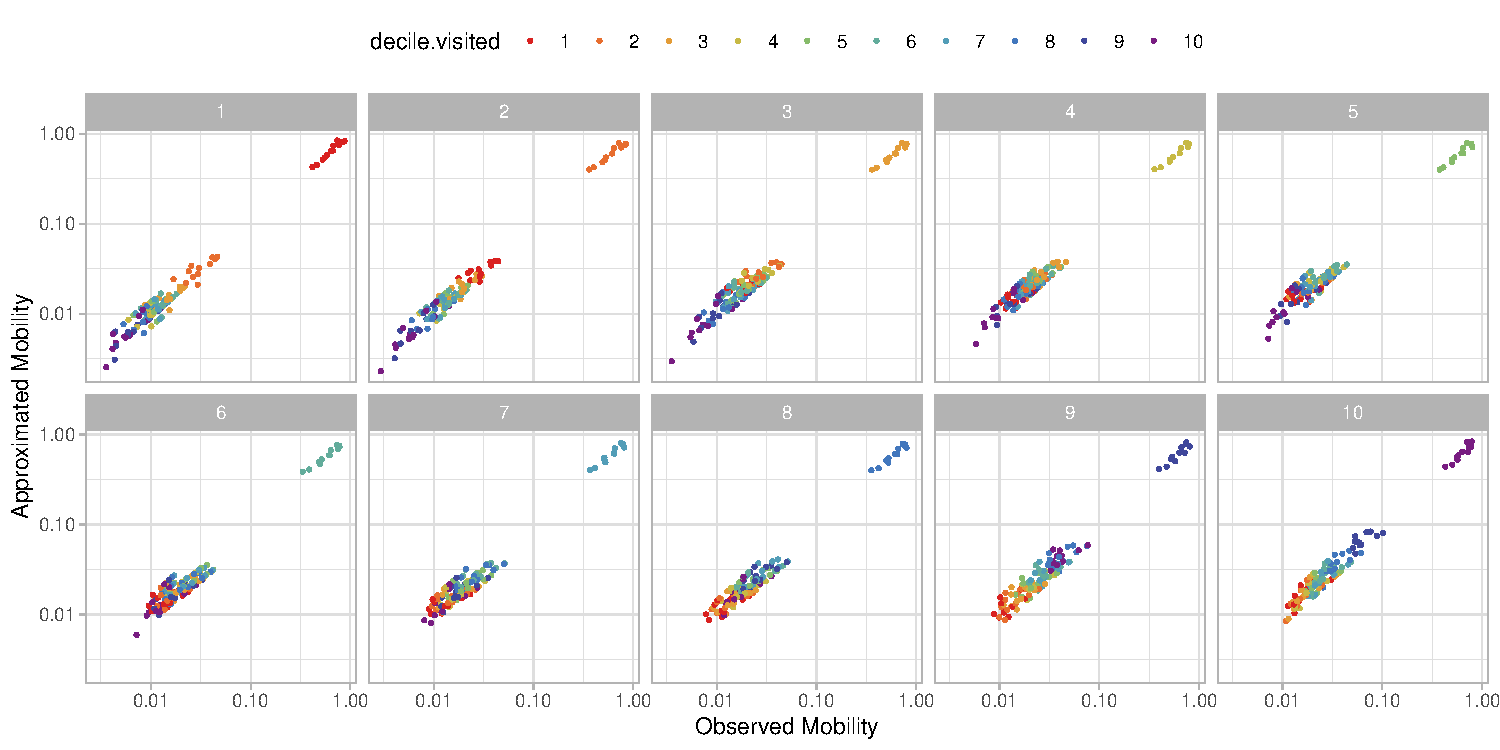
\includegraphics[width=\linewidth]{B-vs-Ba}
  \caption{Comparison of element values ($g$, panels; $g'$, colours) in the
    observed mobility matrix $B_{gg't}$, Eq.~(\ref{eq:Bgg.t}) and
    approximated mobility matrix, Eq.~(\ref{eq:Bgg.t.approx}),
    showing close agreement}
  \label{fig:B.vs.Ba}
  \floatfoot{Derived from mobile device geolocation data;
    deciles represent groupings of Ontario forward sortation areas (FSAs)
    by cumulative \covid cases between 15 Jan 2020--28 Mar 2021;
    scales are log\textsubscript{10} transformed to improve perception of smaller values}
\end{figure}
\clearpage
% ==================================================================================================
\subsection{Additional Data for Ontario Patches}\label{app.covid}
\begin{figure}[ht]
  \centering
  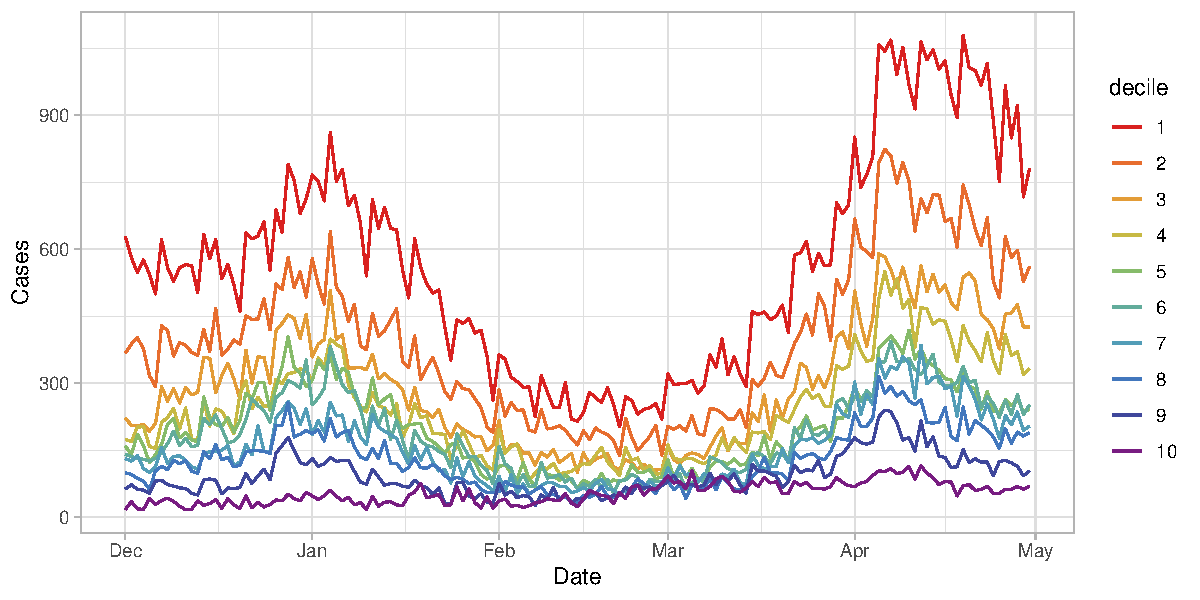
\includegraphics[width=.8\linewidth]{Yg}
  \caption{Time trends in daily \covid cases across the 10 deciles (patches) in Ontario}
  \label{fig:Yg}
  \floatfoot{Deciles represent groupings of Ontario forward sortation areas (FSAs)
    by cumulative \covid cases between 15 Jan 2020--28 Mar 2021.}
\end{figure}
\begin{figure}[ht]
  \centering
  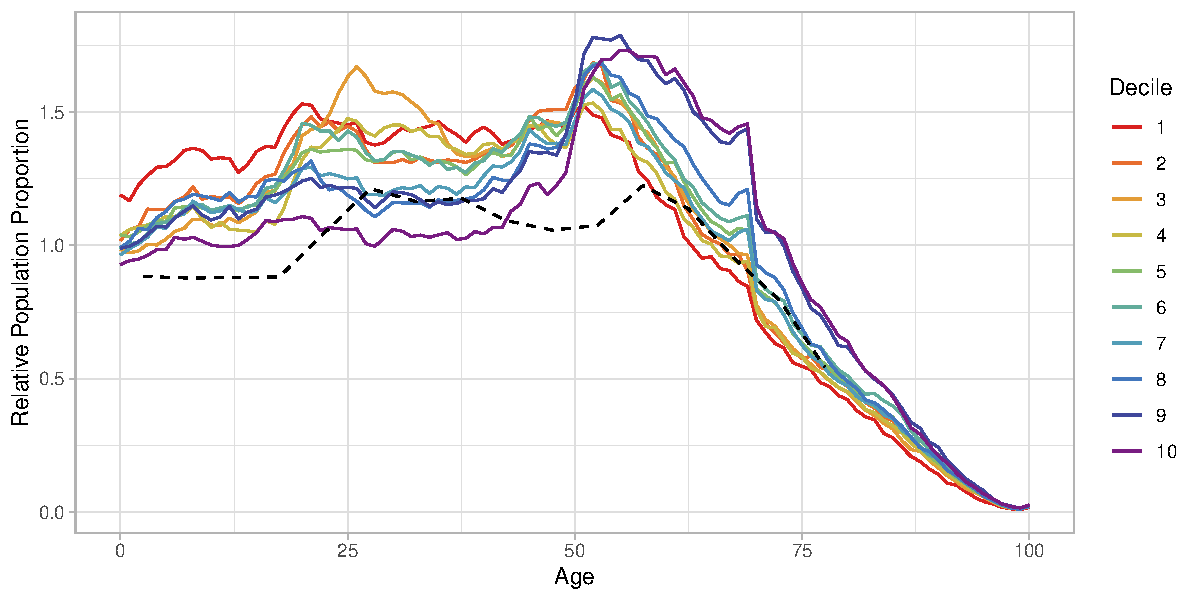
\includegraphics[width=.8\linewidth]{Pga}
  \caption{Population age distributions across the 10 deciles (patches) in Ontario}
  \label{fig:Pga}
  \floatfoot{Deciles represent groupings of Ontario forward sortation areas (FSAs)
    by cumulative \covid cases between 15 Jan 2020--28 Mar 2021;
    solid coloured lines correspond to deciles;
    dashed black line corresponds to Canadian age distribution used by \citet{Prem2017}.}
\end{figure}